\RequirePackage{docswitch}
% \flag is set by the user, through the makefile:
%    make note
%    make apj
% etc.
\setjournal{\flag}

\documentclass[\docopts]{\docclass}

% You could also define the document class directly
%\documentclass[]{emulateapj}

% Custom commands from LSST DESC, see texmf/styles/lsstdesc_macros.sty
\usepackage{lsstdesc_macros}

\usepackage{graphicx}
\graphicspath{{./}{./figures/}}
\bibliographystyle{apj}

% Add your own macros here:


\author{Rick Kessler,  Rahul Biswas, Alex Boucard, Mi Dai, Renee Hlozek,
Saurabh W.~Jha, Lluis Galbany, Emille Ishida, Ashish Mahabal, Kaisey Mandel, Rafael Martinez-Galarza, Daniel Mutukrishna, Tina Peters, Kara Ponder}

% ======================================================================

\begin{document}

\title{The Photometric LSST Astronomical Time-series Classification Challenge (PLAsTiCC): Data set}

%\maketitlepre

\begin{abstract}
The Photometric LSST Astronomical Time Series Classification Challenge (PLAsTiCC) is an open data challenge to classify simulated astronomical time series data in preparation for the data from the Large Synoptic Survey Telescope (LSST), that will achieve first light in 2022. We briefly describe the PLAsTiCC data set that will be tested by the Kaggle team. This note will be updated for the full release of the data to the community.

\end{abstract}

% Keywords are ignored in the LSST DESC Note style:
\dockeys{}

\maketitlepost

% ----------------------------------------------------------------------
% 

\section{Introduction}
\label{sec:intro}
PLAsTiCC is a large data challenge where participants are asked to \textit{classify astornomical time series data}. These simulated time series data, or `light curves' are measurements of flux in different astronomical wavelength bands as a function of time, and are simulations of what we expect from the upcoming LSST survey. For each object, the data provided includes summary data about the object: its position on the sky, an estimate of its observed redshift (which correlates with its distance away from us), and other properties of the sky near the object. In addition, the \textit{photometry} information on the object is a table of fluxes at different times of observation.

In Figure~\ref{fig:lc}, we show two light curves for different types of objects.

\begin{figure*}[htbp!]
\begin{center} 
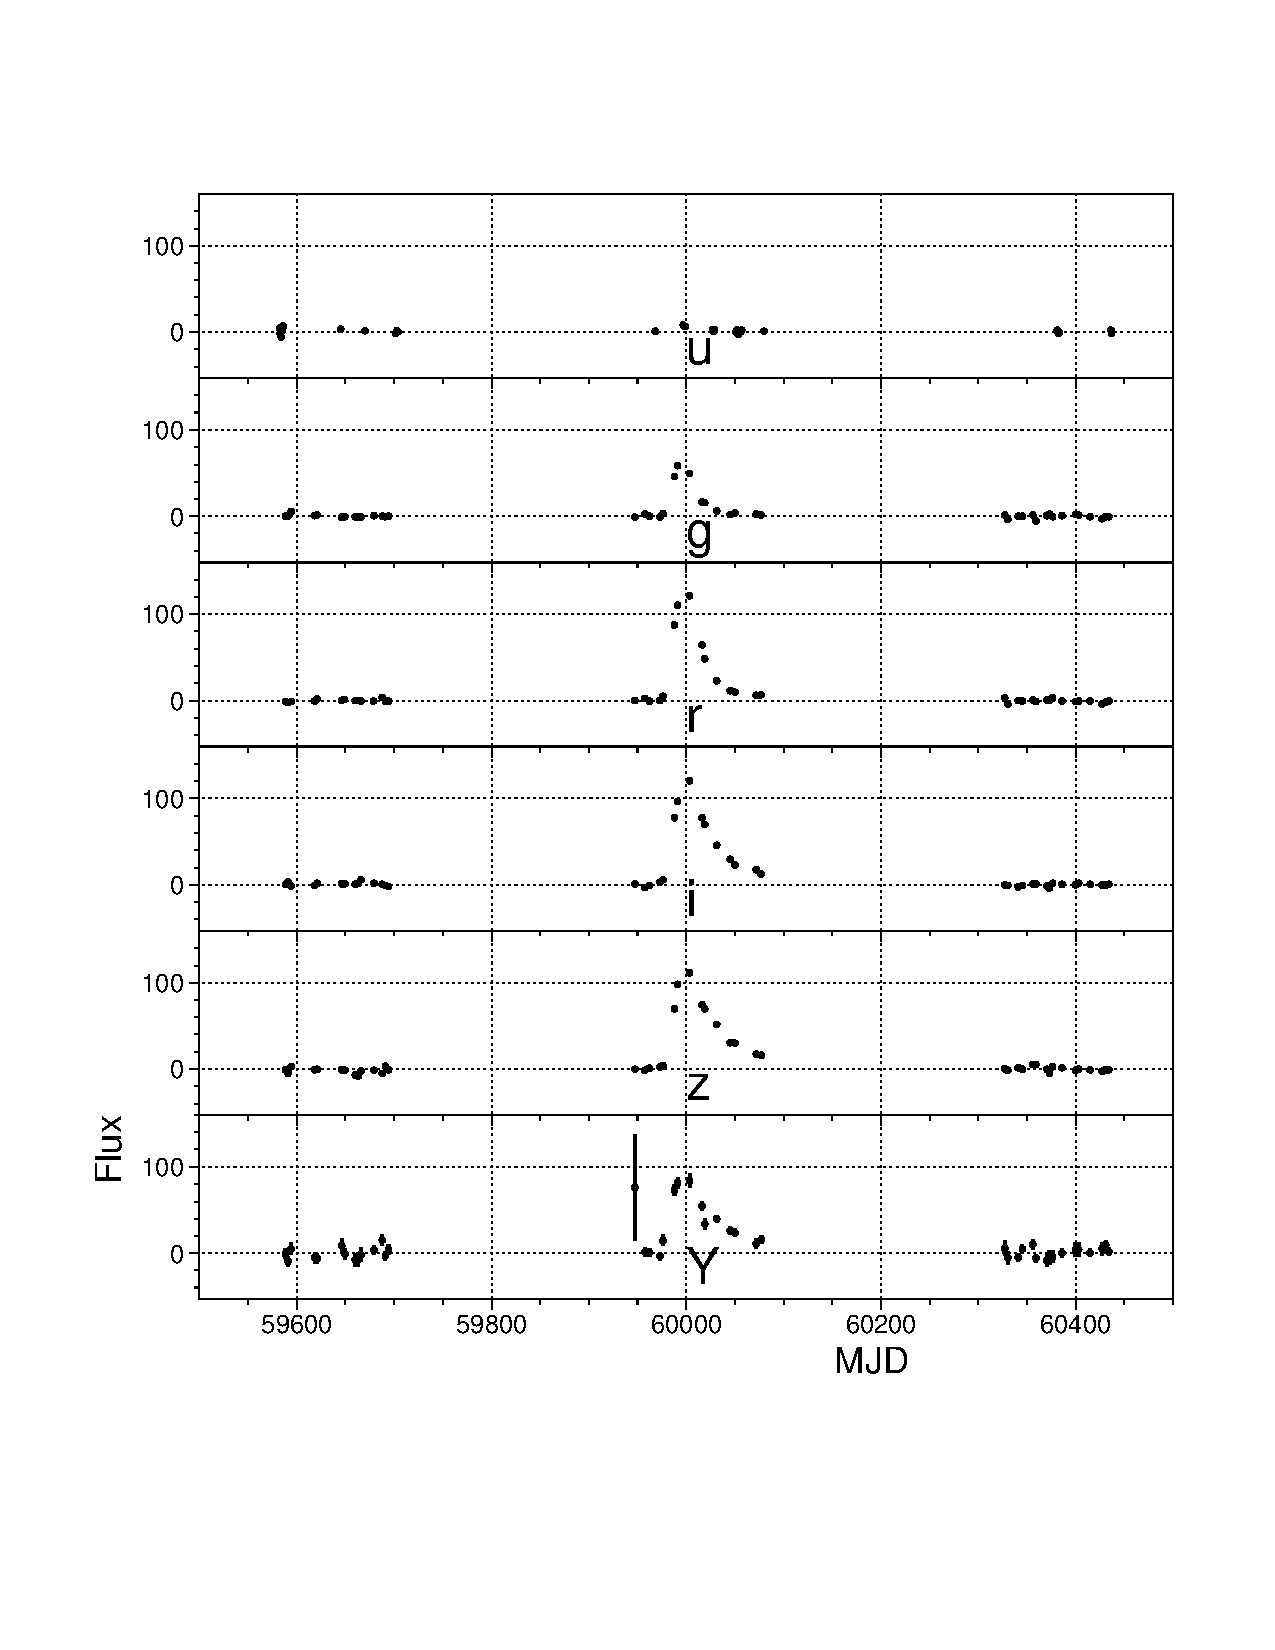
\includegraphics[scale=0.4, trim = 15mm 45mm 10mm 20mm, clip]{figures/lcplot_model01a.pdf}
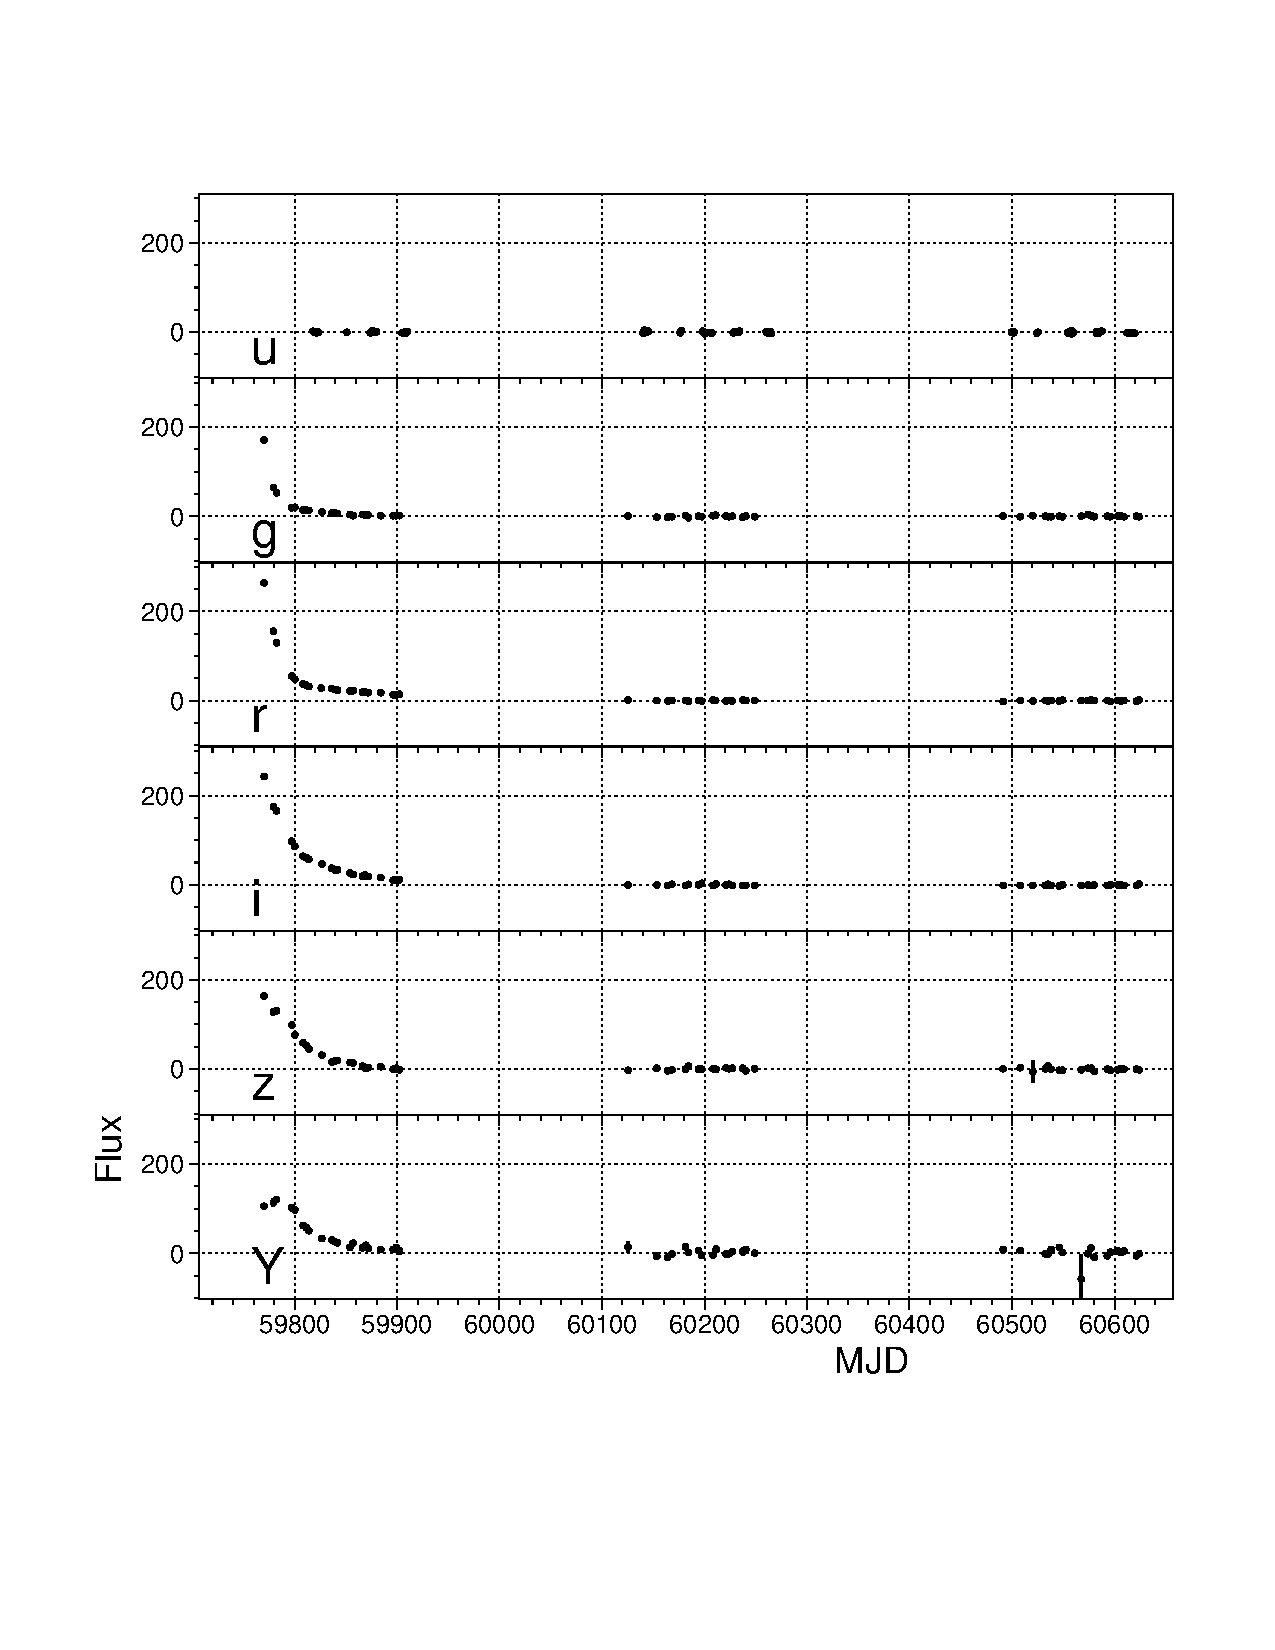
\includegraphics[scale=0.4,trim = 15mm 45mm 10mm 20mm, clip]{figures/lcplot_model01b.pdf}
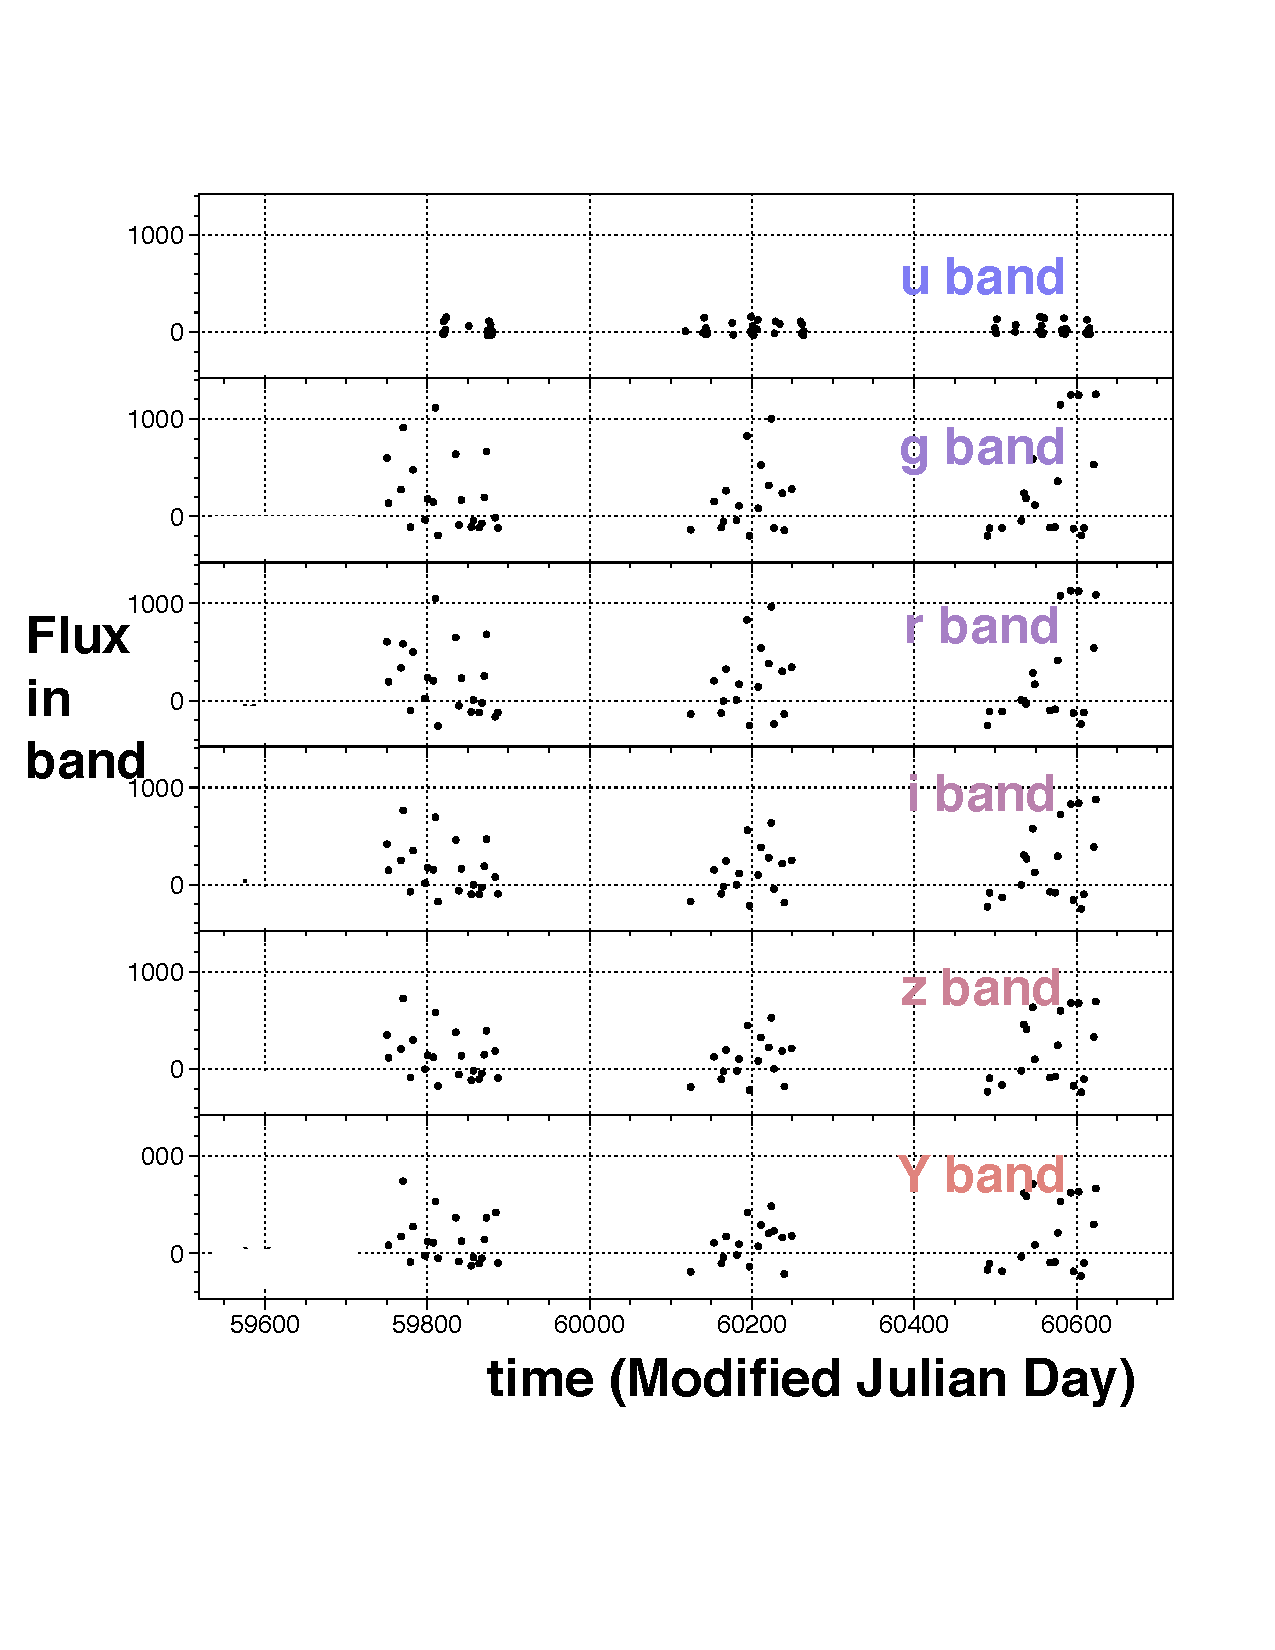
\includegraphics[scale=0.4,trim = 15mm 45mm 10mm 20mm, clip]{figures/lcplot_model80.pdf}
\caption{Example light curves in the PLAsTiCC data set. The three example objects display different changes in flux with time typical of real-world objects. They are either transient, and brighten suddenly before fading again into obscurity (top row) or they display flux variability, brightening and fading (bottom figure). This brightening can either be periodic or aperiodic. The top row also illustrates that the brightening of the flux can occur near the edges of the survey, and therefore may not include the full time period of brightening for the object. In addition, all three panels show that seasonal gaps and the instrument cadence of observations can introduce gaps in the light curve.\label{fig:lc}}
\end{center}
\end{figure}
The users are asked to classify the data into XX classes, XX-1 of which are reprsented in the training sample. The final class designation of `other' is meant to capture objects that have not been seen into one class.


\subsection{Astronomy Background}
While we think of the night sky as static, it is filled with sources of light that vary in brightness on timescales from seconds and minutes to months and years. 

Some of these events are classified as \textit{transients}, and can be the
observational consequences of a large variety of astronomical phenomena. For example, the cataclysmic event that occurs when a supernova explodes generates a bright signal that fades with time, but does not repeat.

Other events are classified as \textit{variables}, since they can vary their brightness in a periodic (or aperiodic) fashion, and originate from physical process governing high density regions of the Universe such as emission from the active galactic nuclei (AGN) at the hearts of galaxies, or our position in relation to a set of observed objects (e.g. eclipsing binaries).

These relatively rapid changing objects can provide important clues about themselves and their environement - as well as the evolution of the universe as a whole (e.g. type Ia supernovae provided the first evidence of the current accelerated expansion of the Universe caused by dark energy). Crucially, the different types of transients and variables, given \textit{different} pieces of information, and therefore, the proper classification of transients is a crucial task in observational astronomy - specially in the light of large data volumes expected for the next generation of astronomical surveys.

The main aim of this challenge is: \textit{can one classify astronomical transients and variables from a photometric data set designed to mimic the data from the upcoming Large Synoptic Survey Telescope (LSST)?} Crucially, the classification will occur on a large test set, but the training data will be a small, and poorly representative training set, to mimic the challenges we face observationally.

We now give more detail on LSST, and the challenge at hand. The two modes for characterising the light from the objects, are called spectroscopy and photometry.

Spectroscopy is the modern equivalent of using a prism to separate a beam of white light in its composite (e.g. rainbow) colours. It is a high resolution measurement which allows us to identify any emission/absorption features indicative of specific chemical elements present in the object - and are also the main source of information enabling classification. Despite being paramount for the classification task, spectroscopy is an extremely time consuming process - with integration times hanging from 20 minutes to a few hours depending on the telescope and brightness of the source.

Traditionally, classification is completely based on spectroscopic measurements - however, given the volume of data expected from the upcoming large scale sky surveys, this strategy is not sustainable. An alternative approach, based on cheaper/lower resolution measurements must be found. The spectra are described as flux per wavelength interval. 

Different physical processes (and chemical elements) are found at different wavelengths of the spectrum, and so different parts are useful to distinguish between objects.

Photometry is gives the overall information of how bright the source is (how much energy the object is emitting) at a particular moment. It can be described as the low resolution counterpart of spectroscopy - or the integral of all the information stored in the spectra. The resultant photometric magnitudes $m$ are related to the flux in a given (average) wavelength through 
\begin{equation}
F = 10^{-0.4m+11} + \mbox{noise}
\end{equation}

These band fluxes are the integrals of the appropriately redshifted spectrum over the filter bandpasses of atmosphere and the instrument divided by the energy of photons in the central wavelength of the filter. A sequence of photometric observations made at different times is called a light curve. It holds the information of how the energy of the source evolves with time and can also be used to characterize different types of supernovae (although the distinction between classes is much more discrete than we would hope it to be). As a consequence, for each object we will have a number of light curves in each filter (or band). For LSST, the filters are the $ugrizy$ filters and are roughly 1000 Angstrom wide, spanning a range from 3000 Ang to 9000 Ang. The observations are noisy, mostly because of sky noise which is due to light form different components, and this varies with time (eg. twilight, effect of the moon) and its strength is different in different bands. Therefore the bands will vary in usefulness for different objects. In addition, the bands are sensitive to different physical processes in the same way as the spectrum, and so will be more or less useful to distinguish between objects.

In addition to being more cost effective, it is possible to obtain photometry of objects to greater distances (and volumes) in the universe. For an object of given brightness (luminosity), the flux received on earth decreases with the distance to the object as
\begin{equation}
F = \frac{L}{4\pi d_L^2}.
\end{equation}


%Hence if the intrinsic luminosity of an object is known, then its flux can be used to determine the distance to the object. This distance is an important tool in classification, since different objects are more likely to be found within or outside of our own galaxy.

%When working in magnitudes, we connect the distance to the magnitudes via the distance modulus $\mu$:

%\begin{equation}
%\mu = m-M = 5\log_{10} d_L + 25,
%\end{equation}

%where $M$ is the (unknown) intrinsic brightness of the object, $d_L$ is measured in megaparsec (Mpc), $c$ is the speed of light and $H_0 \simeq 70$ km/s/Mpc is the Hubble constant. Programs exist to fit for the distance modulus $\mu$ given the light curve points and models for the type of object.

New instruments, like the Large Synoptic Survey Telescope (LSST) - scheduled to begin observations in 2022 - will produce an unprecedented number of light curves. Once these transients are detected, we rely on agreements with other telescopes in order to acquire a small number of spectroscopic observations.

The final connection to a model of the cosmology of the universe, and the distances to objects comes through the redshift, $z$. Redshift is an emperical quantity that is defined by measuring the difference in the observed wavelength $\lambda_o$ of a given feature (e.g. in the spectrum described above) compared to the emitted wavelength $\lambda_e$, or

\begin{equation}
z = \frac{\lambda_o - \lambda_e}{\lambda_e}.
\end{equation}

 It is the light analogy of the Doppler effect that we are used to in sound. It is clear then that using a spectrum to determine the redshift of an object gives the most precise result (with the smallest error $\sigma_$). However photometry can also be used to determine a redshift for an object, the so-called photometric redshift, with a larger uncertainty. Given that photometric error relies on prominent features moving between the (large) bandpasses, it is also possible to insert `catastrophic' redshift error, where the redshift of the object is misassigned. These errors are rare (roughly $2\%$ of the total number of objects), however can pose serious problems for classification of objects.

The distance modulus is connected to the cosmology as a function of redshift $z$ and the components of the universe. We do not expect participants of this challenge to compute these functions, and will provide the distane modulus and error on the modulus as if the data had been run through a light-curve model fit.

We will describe the data in the following sections, and discuss the metrics used to classify objects in a separate note.
\section{The data}
\label{sec:thedata}
The lightcurve data is made of non-homogeneously sampled, non-periodic time series with correlated errors obtained in several wavelength filters.

A database over all objects will be provided. The following data are provided:

\begin{itemize}
\item {\tt objid}: the Object ID
\item {\tt ra, dec}: right ascension and declination (the sky co ordinates of the object) (???)
\item {\tt mwebv, mwebverr}: the value of the Milky Way extinction at that position on the sky, and its associated error
\item {\tt specz}: the spectroscopic redshift
\item {\tt photoz, photozerr}: the photometric redshift and its respective redshift error (these entries are null for the training set)
\end{itemize}

It will also contain a table of photometry with the following information:
\begin{itemize}
\item {\tt mjd}: the Modified Julian Date (MJD) of the observations
\item {\tt pb}: the Petrosian brightness, a measurement of the signal to noise of the measurement
\item {\tt flux}: the measured flux in each of the LSST bands
\item {\tt fluxerr}: the error on the measured flux in each of the LSST bands
\item {\tt photflag}: photometry flag, which indicates the quality of the object (eg. it will be flagged if observations have saturated)

As part of the challenge, we provide a Jupyter notebook to read in the data, and a notebook to compute the metrics for the challenge.
\end{itemize}

The training set will also contain the simulated model name, while the test data will not: it is the task of those participating to determine the classification flag of the test set.

\subsection{Training data}
The training data will be a subset of $\sim 5000$ objects taken from the larger test data set. The relative rates of the data will be adjusted slightly in the training sample. In addition, the test data will contain some rare objects that are not seen in the training data. The final classification classes will therefore contain an `other' class to be used on any object that the classifiers have not seen before.



% ----------------------------------------------------------------------

\section{Challenge participation}
\label{sec:conclusion}
PLAsTiCC participants must return an $M\timesX$ table of classification probabilities, where $M$ is the number of objects in the test dataset, and $X$ is the number of classes, including the `other' class. The row entries sum to unity, to ensure normalised probabilities. The winner of the challenge will be the person who maximises the PLAsTiCC metric score (which is described in a separate note included in this challenge). 

While some members have been shielded from information about model specifics, the PLAsTiCC team involved in validating the data will not be able to participate in the challenge directly, and will only publish classifications on the data once the challenge has completed.

% ----------------------------------------------------------------------

\subsection{Acknowledgments}
The PLAsTiCC data relies on the inclusion of a host of models of astronomical transients and variables. These will be outlined in a paper to be published once the challenge is complete. While we cannot thank them by name at this stage (as this would no doubt identify the models included in the challenge)  we acknowledge their contributions anonymously at this stage. This work was supported by an LSST Corporation Enabling Science grant, and a Dark Energy Science Collaboration Workshop support grant.

%%% Here is where you should add your specific acknowledgments, remembering that some standard thanks will be added via the \code{desc-tex/ack/*.tex} and \code{contributions.tex} files.

%This paper has undergone internal review in the LSST Dark Energy Science Collaboration. % REQUIRED if true

%
 % Standard papers only: author contribution statements. For examples, see http://blogs.nature.com/nautilus/2007/11/post_12.html

% This work used TBD kindly provided by Not-A-DESC Member and benefitted from comments by Another Non-DESC person.

% Standard papers only: A.B.C. acknowledges support from grant 1234 from ...

\input{desc-tex/ack/standard} % also available: key standard_short

% This work used some telescope which is operated/funded by some agency or consortium or foundation ...

% We acknowledge the use of An-External-Tool-like-NED-or-ADS.

%{\it Facilities:} \facility{LSST}

% Include both collaboration papers and external citations:
%\bibliography{main,lsstdesc}

\end{document}

% ======================================================================
